

\chapter{Ongoing projects}
\label{ch:projects}

I don't yet know where to put each of these project sections...

\section{The Drosophila fruitfly project}
Throughout this book we will embed many of the concepts we are discussing within a real-life project, which we will call ``the fruitfly project''. The fruitfly project is a genomics project that I have been involved in with several of my students and my collaborators at Lawrence Berkeley National Laboratory (LBNL).

As most do, the fruitfly project began with a question: ``Is spatial information useful for making gene-gene interaction discoveries?''. To expand and de-code this question for the non-biologists, what the group was really asking is whether it is possible to use stained images (more specifically, images of Drosophila embryos) to identify whether genes interact with one another. For an individual embryo, the staining process involves using dye to stain specific products that are produced when a particular gene is being expressed (these products are typically proteins). The upshot of the staining process is that areas within the embryo where the stain is visible correspond to physical locations within the embryo where the gene of interest is being expressed. 



With this question in mind, the group of biologists at LBNL had generated 1640 spatial gene expression images (see Figure~\ref{fig:embryo}) representing 755 genes for early \emph{Drosophila} embryos. In each image, the gene of interest is being expressed at the locations within the embryo where the blue stain is visible. Each processed expression image can be represented by a numeric vector with 405 entries, one for each of the 405 pixels inside the ellipse template.





\textcolor{red}{So the biologists had the data and the question but no idea how to answer it? They then invited Bin and co. to offer statistical insights whereby after much trial and error, we arrived at the non-negative matrix factorization approach. This approach allowed us to derive 21 principal patterns (PPs) using which we constructed spatially local correlation networks for all patterned transcription factors during early Drosophila development}

% img source: http://insitu.fruitfly.org/cgi-bin/ex/report.pl?ftype=1&ftext=TE18870

\begin{figure}[H]
\begin{center}
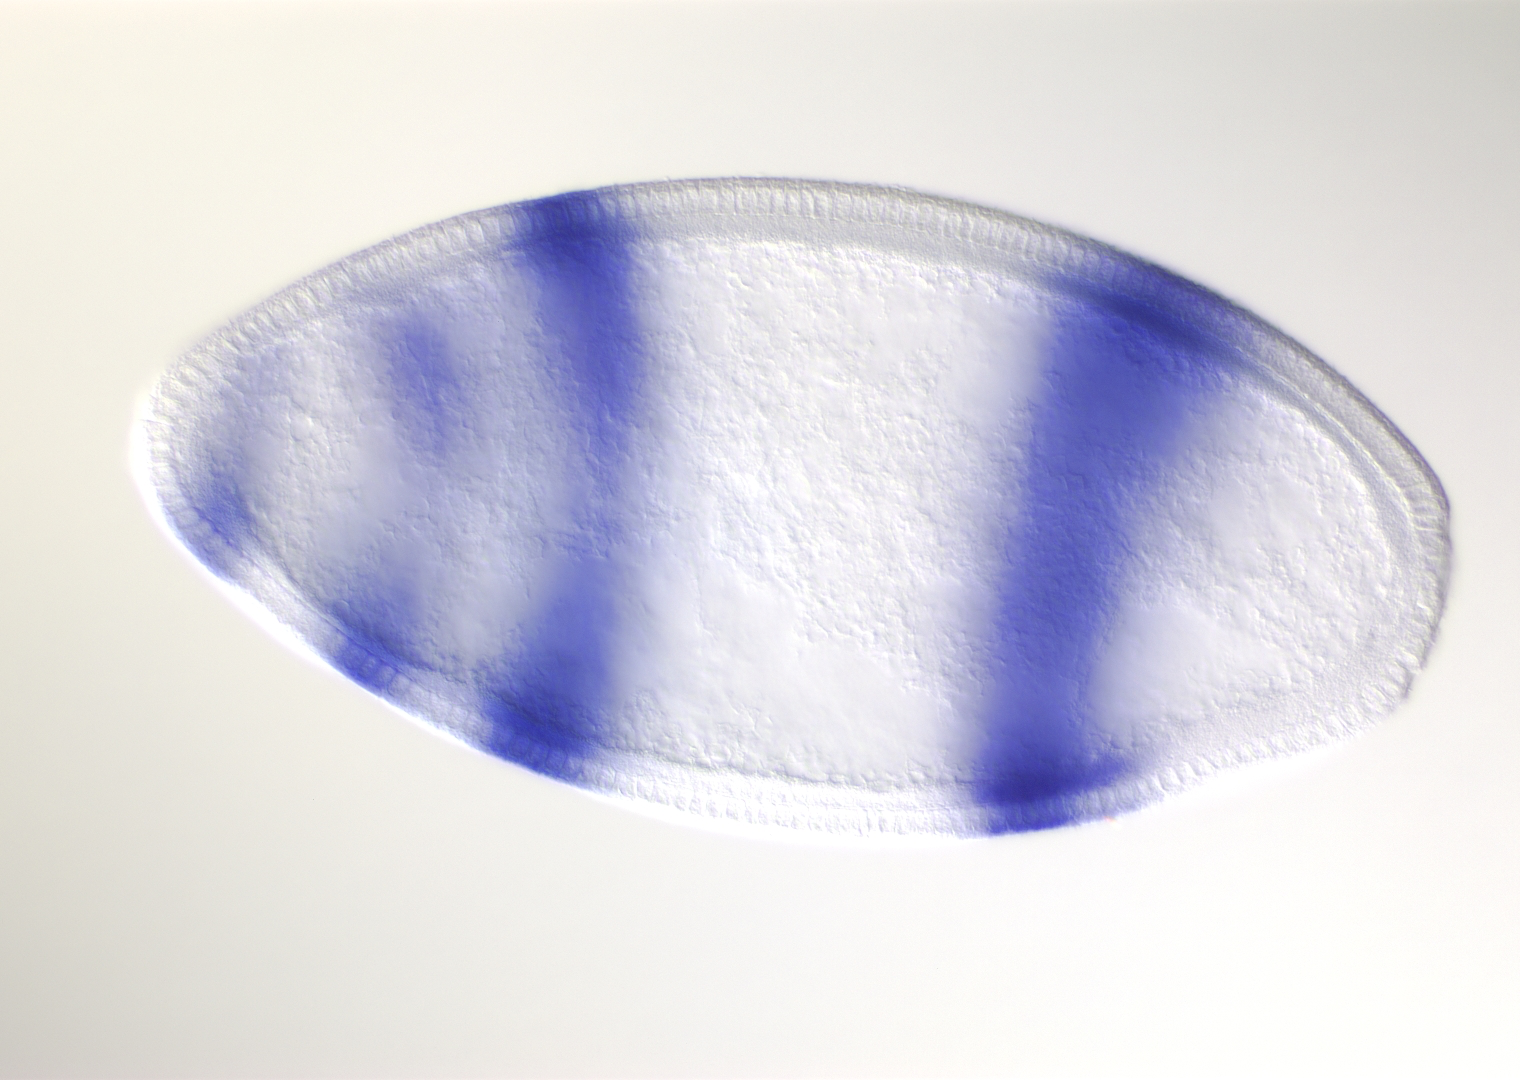
\includegraphics[scale=0.15]{embryo.png}
\end{center}
\caption{An example of drasophila embryo for which the blue stain corresponds to the regions of the embryo in which the \emph{giant} gene is being expressed.}
\label{fig:embryo}
\end{figure}


\subsection*{The gap gene network}

The gap gene network consists of a group of interacting genes each of which are involved in the process of segment determination in the early development stages of the fruitfly. discovered by Nobel Prize winners Christiane N\"{u}sslein-Volhard and Eric Wieschaus in 1980. The term ``gap'' arose as a result of the effect of mutations of these genes on the embryonic development: gap genes cause the loss of central segments from the embryo which results in gaps in the developing structure.

Examples of these genes include \emph{kr\"{u}ppel}, whose early expression domain is in the center of the embryo, which, along with \emph{knirps} and \emph{giant} are among the earliest genes expressed during development. These genes subdivide the embryo along the anterior/posterior axis (the longest axis).


\begin{figure}[H]
\begin{center}
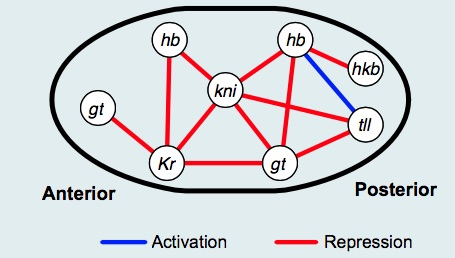
\includegraphics[scale=0.5]{gap_gene.jpg}
\end{center}
\caption{The gap gene network}
\label{fig:gap}
\end{figure}




In Figure~\ref{fig:gap} above, we see a network of 8 gap genes each of which have activation or repression effects on one another. For example, \emph{gt} (giant) and \emph{Kr} (Kr\"{u}ppel) repress one another in the sense that if \emph{Kr} is being highly expressed, then \emph{gt} will be less expressed. \emph{hb} (hunchback) and \emph{tll} (tailless), on the other hand, activate one another whereby increased expression of one of the genes activates increased expression of the other.


\begin{figure}[H]
\begin{center}
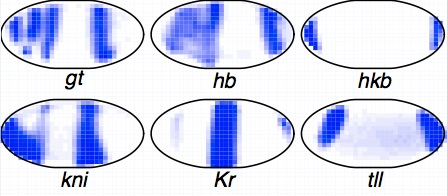
\includegraphics[scale=0.5]{embryos.jpg}
\end{center}
\caption{Expression regions for each of the gap genes}
\label{fig:stains}
\end{figure}


Figure~\ref{fig:stains} presents examples of embryos for which the product of the expression of each corresponding gap gene is dyed blue. That is, each image shows us the locations where (and extent to which) each gap gene is being expressed. We see that the \emph{Kr} (Kr\"{u}ppel) gene is expressed in the mid-region of the embryo, while \emph{hkb} (huckebein) gene is expressed only at the posterior and anterior ends. We also see that although there are regions of complementary expression, for example \emph{gt} and \emph{hb} have complementary expression patterns towards the right end of the embryo, implying that their local correlation is negative.





\subsection*{The experiment}

When we stained the products of the expression of \emph{new genes} with unknown functions in our embryos, we were able to use the images to identify whether these new genes interacted with the known gap genes.


\begin{figure}[H]
\begin{center}
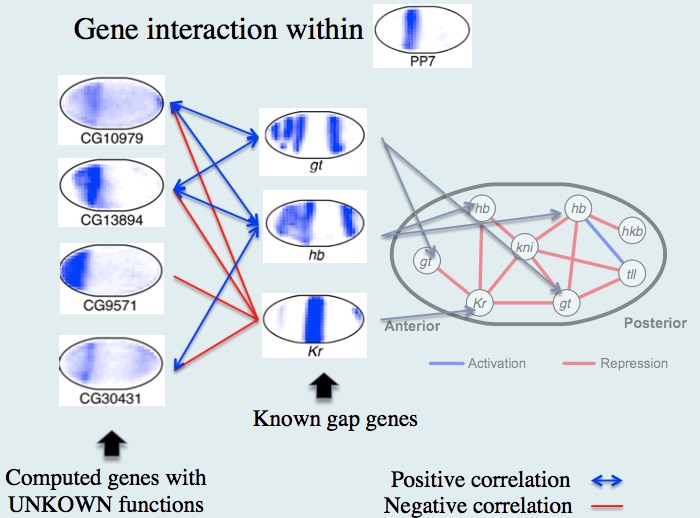
\includegraphics[scale=0.5]{embryos1.jpg}
\end{center}
\caption{Our new CG genes and the gap gene network}
\label{fig:embryo_gap}
\end{figure}



What we found was that our new genes (CG genes) interacted with the famous gap gene network. For example, two genes are positively correlated if they are expressed in the same location in the embryo (the genes have an activation relationship), and negative correlation if they are expressed in non-overlapping locations (the genes have a repressive relationship).

So the question became, are these new genes (focusing on the CG13894 gene) part of the gap gene network?

To answer this question, gene knock-out experiments were carried out by Ann Hammonds in Celniker's lab at LBNL. This is an experiment with an \emph{intervention}: in some embryos, we ``knock-out'' the gene of interest and observe the difference between the development of these embryos and normal embryos. This can be seen as a randomized experiment from which we can try to draw causal inferences \textcolor{red}{What are we trying to infer that knocking out this gene causes?}.

Our local analysis predicted that knocking out CG13894 would cause a change in the gap between the first two stripes \textcolor{red}{(what are these stripes -- is this still staining gene expression or is this just segmentation)}


We formulated this into a hypothesis that asked: ``Will knocking out CG13894 cause a narrowing in the gap between the first two stripes?'', a well formed question that we could assess using a randomized experiment: from our sample of embryos, we could randomly select a certain number to undergo the knock-out process (the treatment embryos) and allow the remainder to develop naturally (the control embryos). We could then compare the gab between the first two stripes between the two groups of embryos. Seems straight forward right? Maybe not... First of all, how can we quantitatively compare the gap between the stripes in a reliable way (i.e. other than by simply looking at them)?




\begin{itemize}
\item {\bf The first approach}: measure the gap between the stripes within the image. But embryos come in all different shapes and sizes! Recall our data wisdom section on ensuring comparability between our units of analysis. Comparability is extremely important in this situation, otherwise we have a confounding factor which is the size of the embryo. 
\item {\bf The second approach}: count the number of cells in the gap between the stripes. How could we automatically count the number of cells in images of this resolution? We had to manually count the number of cells which is tedious. Further, the count may be different at different ages, since as the development progresses, the cells divide, so we may just be counting the age of the embryo! Further, what if the change in the gap is a result of the cell size changing instead of the number of cells. Then this measure would be useless.
\end{itemize}




Even in measuring this gap, there are a lot of judgement calls and assumptions that come into play. For example, should we normalize? Stripes from each embryo are of different thicknesses and perhaps we should be considering the size of the gap relative to the size of the stripes for each embryo. The histograms below show the distances first when we do not normalize and then after normalizing relative to the size of the first stripe (the ratio of the size of the gap to the size of the stripe).


\begin{figure}[H]
\begin{center}
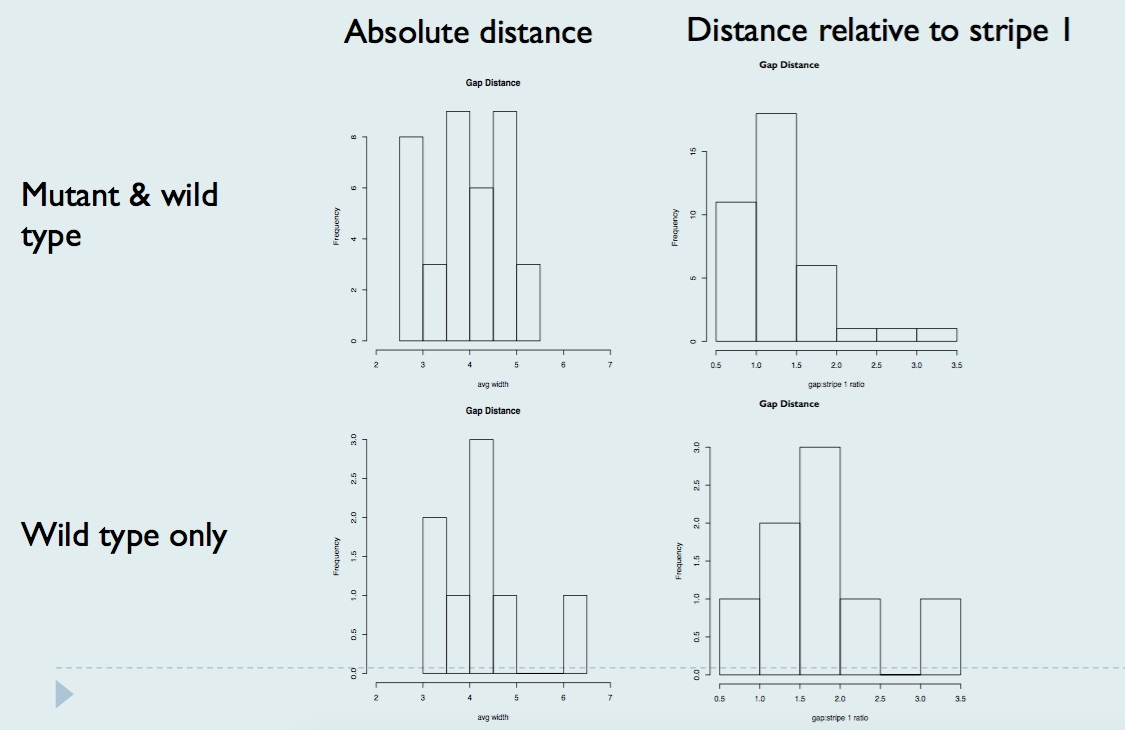
\includegraphics[scale=0.25]{gap_width.jpg}
\end{center}
\caption{Histogram of gap widths}
\label{fig:gap_widths}
\end{figure}



Perhaps you might now think about a few of our data wisdom questions from the previous chapter and apply them to this project:

\begin{enumerate} 
\item What does a number in this dataset mean? It is often not discussed enough what numbers are you actually interested in. Do the numbers you have actually measure what you're interested in. If you're using the wrong numbers, then you either don't see anything or you see things that aren't really there. We discussed above different types of ``numbers'' that we could have used for the distance. Some would have been more effective than others for detecting a real difference between the knock-out embryos and the control embryos.
\item Eventually you'll find a difference between the mutant and normal embryos. When this occurs, how can you test to see if this difference is real and not just an artefact of the data you have or the model you used? Instead of worrying about this problem at the end, it is always a good idea as soon as you've collected your data to set aside some subset (half?) of the data and don't use it for any of your analysis (this witheld subset of your data is called the \emph{test data}). You don't want to ``over-snoop'' the data. When you have a finding based on your training data, you can test to see whether the results are also true in the test data.
\item How was the randomization done in this experiment? We told you that the embryos were randomized to either undergo the knock-out procedure or not, but we didn't tell you how this occurred. 
\item What is our overall population? What are we assuming about the population? The embryos have all been bred in the lab and come from a particular genetic lineage. The population about which we are making inferences is not simply \emph{all fruitflies} in the world, or even in Berkeley. Even amongst the fruitflies at the lab, there is not overall homogeneity. Each embryo is different.
\item How was the knock-out ``intervention'' performed? It's certainly not possible to simply manipulate each individual fruitfly. Typically you perform the knock-out intervention in a few fruitflies and they pass the mutation on to their offspring. This process probably also resulted in many of the fruitflies dying, in which case, is there a difference between those who survived and those who died in terms of how extreme the gap difference would be?
\end{enumerate}
 
 
 
\section{The neuroscience project}
 
 
\subsection*{Neuroscience: Hubel and Wiesel's cat experiment}

Hubel and Wiesel (1959) conducted some of the pioneering research in showing how the visual system constructs complex representations of visual information from simple stimulus features. In one of their most notable experiments, they anesthetized a cat and propped its eyes open, so that the cat was physically seeing things, but was not conscious. They inserted a microelectrode into the primary visual cortex of the cat and they projected bright patterns (circle, line) on a dark screen in front of the cat. What they found was that some neurons fired rapidly when presented with lines at one angle, while others responded best to another angle. 


% https://goodpsychology.files.wordpress.com/2013/03/hubel-experiment.jpg

\begin{figure}[H]
\begin{center}
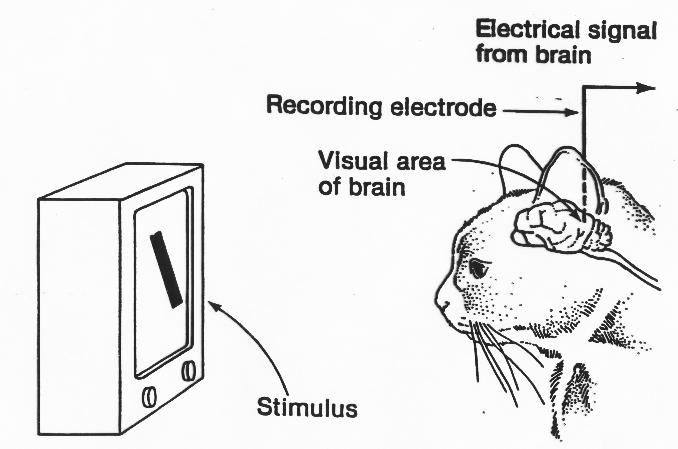
\includegraphics[scale=0.25]{hubel.jpg}
\end{center}
\caption{The Hubel and Wiesel cat experiment}
\label{fig:cat}
\end{figure}



This can be interpreted as a causal inference problem: placing the bright object in the line of view of the cat \emph{caused} the neurons to fire. This influential work was described by Professor David Ottoson of the Karolinsksi Institute as

\begin{quote}

``The signal message that the eye sends to the brain can be regarded as a secret code to which only the brain possesses the key and can interpret the message. Hubel and Wiesel have succeeded in breaking the code''
\end{quote}


There has been a recent new wave of research interest in the area of understanding how the brain processes visual stimuli, particularly utilizing deep learning algorithms. A modern direction that developed from Hubel-Wiesel's work in the way in which we computationally preprocess images for analysis. We use \emph{Gabor filters} to model simple cells in the visual cortex, so Gabor functions can be thought of as the mathematical representation of the perception in the human visual system.

Gabor filters (see image below) correspond to functions which represent the particular spatial frequencies, locations and orientations that were discovered by Hubel and Wiesel's cat experiment in 1959. When analyzing images, it is very common to decompose the image into the gabor functions for analysis.

\begin{figure}[H]
\begin{center}
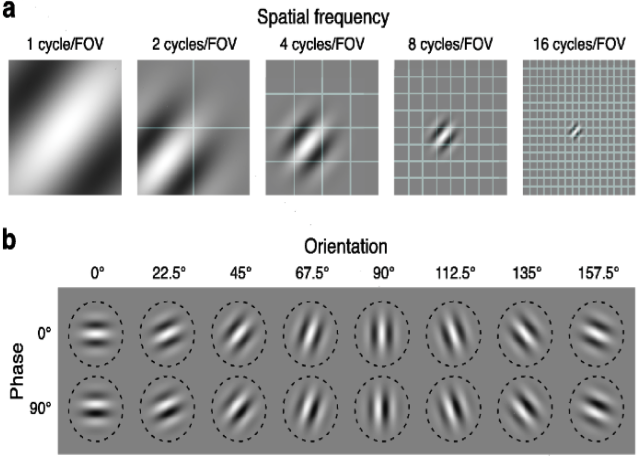
\includegraphics[scale=0.5]{gabor.png}
\end{center}
\caption{Gabor wavelets}
\label{fig:gabor}
\end{figure}


\subsection*{Movie reconstruction using fMRI data: The Gallant Lab}


This is a project that I was involved in with Jack Gallant's lab from the Redwood Center for Theoretical Neuroscience at UC Berkeley. The Gallant lab performed a number of functional magnetic resonance imaging (fMRI) experiments, which measure oxygenated bloodflow in the brain. Measuring oxygenated blood flow can be considered as an indirect measurement of neural activity (the two processes are highly correlated). 

fMRI takes measurements for each voxel (the brain is segmented into voxels which are $1 \times 1 \times 1$mm cubes used to segment a brain into voxels in an analagous way to which we can segment an image into pixels), each of which contains hundreds of thousands of neurons. Compare this modern approach to Hubel and Wiesel's cat experiment which was measuring a single neuron firing, we can see that fMRI gives fairly imprecise measurements. However, given that we have billions of neurons, measuring a single neuron tells us little about how the entire brain functions.

Again, the data is visual: from each fMRI experiment, we obtain cross sectional images of the brain and the blood flow in each voxel. We placed three different subjects in an fMRI machine and showed them videos while measuring their brain activity as shown in the image below.

\begin{figure}[H]
\begin{center}
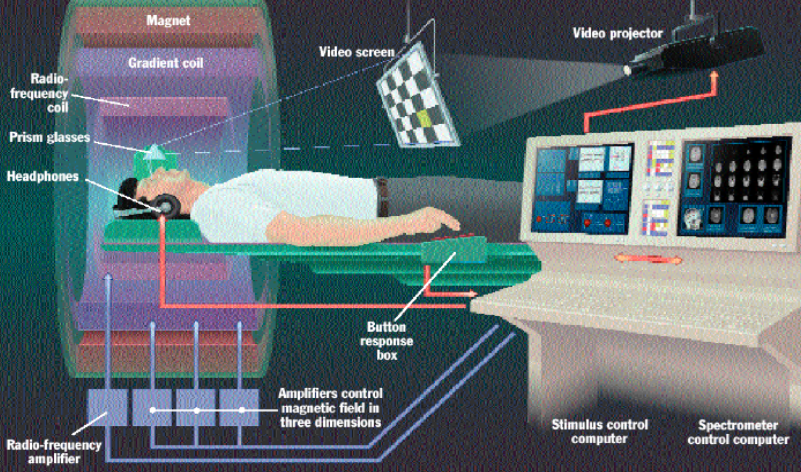
\includegraphics[scale=0.3]{fmri.png}
\end{center}
\caption{An fMRI experiment}
\label{fig:fmri}
\end{figure}

For example, below displays an image viewed by a subject in the fMRI machine and a reconstruction of their brain activity at that moment. The blue regions of the brain shows regions of low activity in the brain and the red regions correspond to high activity \textcolor{red}{(is this right?)}.

\begin{figure}[H]
\begin{center}
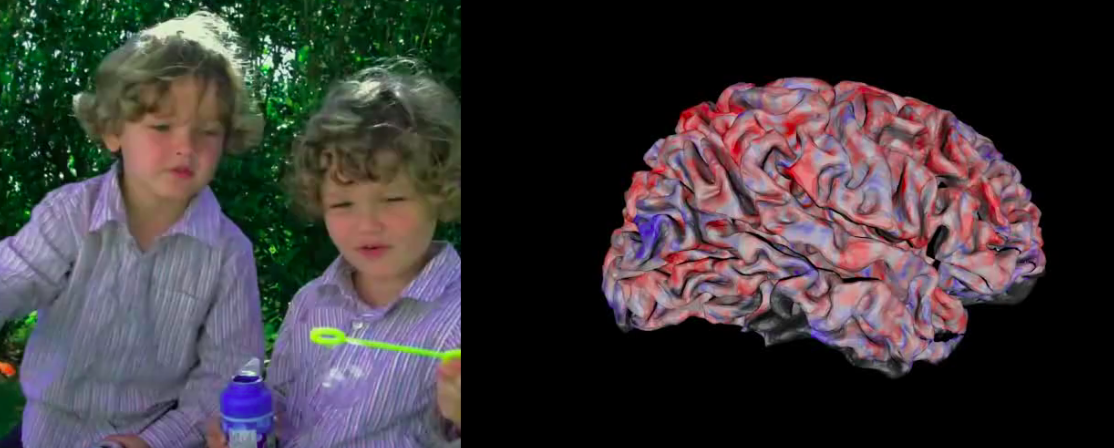
\includegraphics[scale=0.2]{brain.png}
\end{center}
\caption{The brain's response to viewings of an image}
\label{fig:fmri}
\end{figure}


Amazingly, we were able to use fMRI data to reconstruct short segments of film trailers shown to the subjects as the video below shows. There were 7200 seconds of training videos and 5400 seconds of test videos. Some people call this ``mind-reading'' although really it's just data visualization and prediction. \textcolor{red}{give more details of how we did this. It wasn't clear to me from the lecture...}


\subsection*{Predicting brain activity in the visual cortex: The Gallant Lab}

Another project related to that of the fMRI movie reconstruction is the prediction of the brain's responses to visual images as measured in 20 voxels. Recall that fMRI records measurements for discretized 3D volumes of the brain (cube-like regions called voxels), much like an image can be spatially discretized into units of pixels.

For this experiment, the subject is shown pictures of everyday objects, such as a baby, or a house etc. Each picture is a $128 \times 128$ pixel gray scale image, which can be represented by a vector of length $128^2 = 16384$. These image vectors can be reduced to length $10921$ though a transformation based on Gabor wavelets.

Although the actual fMRI response to a given stimulus/image is a function of time, the response of each voxel to each image has been reduced to a single number. The question we are interested in answering using this data is ``do these features/predictors drive the brain signals?''. Once again, we seek a causal relationship.


Given that we have for each voxel response, $10921$ possible predictors from each image, we used the Lasso estimate together with cross-validation (both of which will be discussed later in the book) to identify the most important predictors. That is, for each of the 20 voxels, we are fitting a separate linear model where most of the variable coefficients have been shrunk to zero.

\begin{figure}[H]
\begin{center}
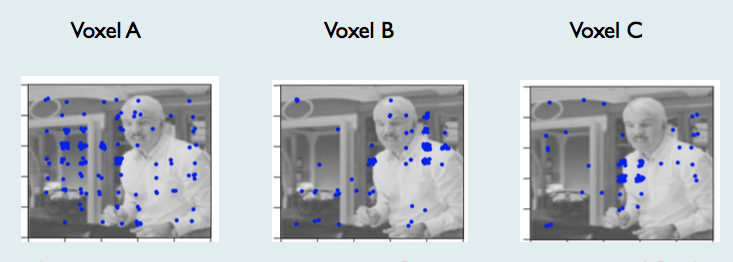
\includegraphics[scale=0.5]{voxel.png}
\end{center}
\caption{The areas within a particular image that are most useful for predicting brain activity}
\label{fig:image}
\end{figure}


For example, in the image above, the blue spots in the left-most correspond to the transformed pixels which are most important for predicting the response for voxel A, and similalry for the responses for Voxels B and C in the two subsequent images.

We could simply accept the variables that the lasso did not shrink, but wouldn't it make sense to actually look at the models being selected over each cross-validation fold?

\begin{figure}[H]
\begin{center}
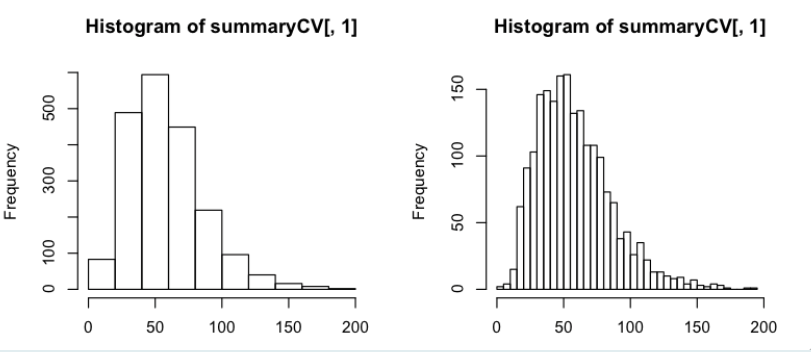
\includegraphics[scale=0.4]{voxelhist.png}
\end{center}
\caption{A histogram of the number of Gabor wavelet features selected by each model}
\label{fig:voxelhist}
\end{figure}

The figure above shows two version of the same histogram describing the number of features selected by each model. It is clear that most of the models select approximately 50 features (by shrinking all other coefficients to 0). The histogram provides us with an overview (by combining all voxels into the same plot) of the models that we have fitted to this data. What have we assumed by visualizing all voxels simultaneously? Primarily, we are assuming that the voxels are comparable to one another, an assumption that seems reasonable. However, it would probably be a good idea to look at the voxels individually as well, since with this combined approach, we might be masking some interesting information corresponding to individual voxels. 

\subsubsection{Assumptions}

It is probably not a reasonable assumption that the voxels are independent to one another, right? But as soon as we don't have independence, some of the most useful models are no longer applicable. Often we assume independence because we don't know how to model the dependence. Most assumptions that we make on our data are assumptions of convenience. Thus the question becomes, if the assumptions of our model are a little bit wrong, how much of an impact will this have on our conclusions drawn from these models? 


Further, what assumptions would we be making by combining the voxel responses from different people? We collected the voxel responses from a number of people, but we chose to analyze them separately. Why? The primary reason is that to combine the data from different people would mean that we had to ensure that the data were normalized (and thus comparable). But how could we do this? In a lot of applied problems, people simply collate their data from different sources together without considering whether this action makes sense.

The issue of normalization is also extremely prevelent in areas of bioinformatics, whereby each run of an experiment has different sources of bias. When the microarray technology first appeared, it was the first time scientists were able to actually look at the expression levels of multiple genes at once. The process of microarray data generation is very physical; someone must fluorescently tag the genes with chemicals and wash away the genetic materials that are not of interest. The data requires so much pre-processing and can be so noisy. \textcolor{red}{Perhaps talk about normalization in terms of microarray data more}. 

It is also common to center the data to have mean zero and standardize so that all observations have standard deviation 1. 







\section{Cloud detection over polar regions}

This project focuses on predicting the presence of clouds in polar regions, which is notable difficult due to the resemblance of clouds to snow from satellite images. Cloud coverage is a key feature of predictive climate models due to the cloud's ability to both act as a blanket to trap heat in the lower atmosphere as well as their ability to reflect rays from the outer atmosphere. Uncertainties about the impact of cloud radiation feedback on the global climate are among the greatest obstacles in understanding and predicting the future of Earth's climate, however the presence of cloud above snow and ice covered surfaces is particularly difficult to detect from satellite images due to the similar reflective and temporal properties of cloud and snow. 

In the late 1990s, NASA launched a satellite called Terra as a part of NASA’s Earth Observing System (EOS), the goal of which is to improve the scientific understanding of global climate changes and provide the scientific basis for environmental policies. Terra was equipped with instruments including a Multi-angle Imaging SpectroRadiometer (MISR), a camera that is used to take pictures of the earth below from multiple angles. NASA's goal for this satellite was to capture images of the Earth each from multiple angles in order to increase understanding of the Earth's systems. At each location, an image is taken from 9 different angles, resulting in images of 9 separate locations. However, as the satellite moves along its path, images of each location are taken from all subsequent angles (see the figure below). Further, each of these images is recorded using 4 different (443nm, 555nm, 670nm, and 865nm Near Infrared Red) wavelengths at each angle.

\begin{figure}[H]
\begin{center}
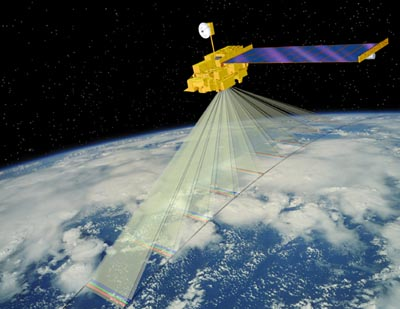
\includegraphics[scale=0.4]{misr.jpg}
\end{center}
\caption{The MISR camera}
\label{fig:misr}
\end{figure}


The MISR algorithm retrieves the cloud height and cloud movement by matching the same cloud in images obtained from three different angles. This algorithm works very well when detecting clouds over darker surfaces such as deep ocean or vegetation covered land surface, but is less effective over snow and ice covered surfaces due to the difficulty in matching.

\begin{figure}[H]
\begin{center}
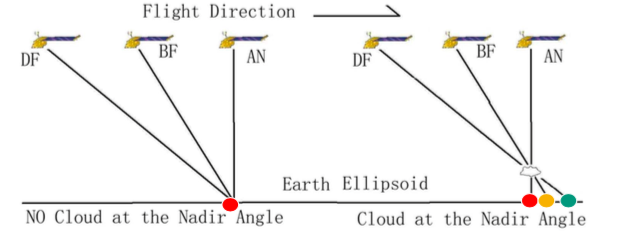
\includegraphics[scale=0.4]{misr_detect.png}
\end{center}
\caption{The MISR camera}
\label{fig:misr2}
\end{figure}

Consider, for example, the figures presented blow. The top panel in the figure below shows a situation in which cloud is easy to detect as it cloud appears over a deep body of water, whereas the second panel displays clouds appearing over ice/snow in Greenland.


\begin{figure}[H]
\begin{center}
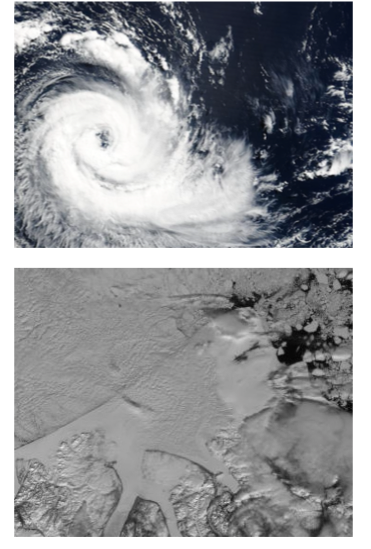
\includegraphics[scale=0.4]{cloud.png}
\end{center}
\caption{Different clouds}
\label{fig:clouds}
\end{figure}



\subsection*{Inital approaches to cloud detection in polar regions: LCMC}

An initial approach (Shi et al. 2002), LCMC, utilizes the domain knowledge that correlations between angles are high over snow and ice covered regions but weak for regions covered by high clouds. Further, clouds are brigher than snow and ice covered surfaces in forward angles (see the figures below). 

\begin{figure}[H]
\begin{center}
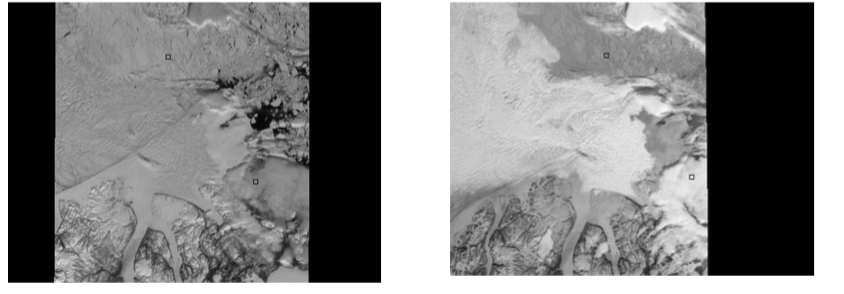
\includegraphics[scale=0.4]{cloud_angles.png}
\end{center}
\caption{Images of clouds over ice regions taken from different angles. The left panel corresponds to the image taken from the AN angle and the right panel corresponds to the image taken from the DF angle}
\label{fig:clouds}
\end{figure}


To utilize this information, this approaches focuses on identifying regions of snow or ice rather than clouds. However, this approach fails in regions where the surface is smooth (such as frozen rivers) or there are thin clouds. How could we adapt the method to rectify these issues? We could use SD to measure smoothness and forward scattering via DF to deal with thin clouds \textcolor{red}{what?}

\subsection*{The Enhanced LCMC algorithm}

The enhanced LCMC algorithn (ELCMC) thresholds 3 features based on 275m, terrain projected red radiances. Instead of utilizing the expert labels, this approach performs clustering (an example of unsupervised learning). The three features are

\begin{enumerate}
\item The correlation between different angles measured by 
$$CORR = \frac{r_{AF - AN} + r_{BF - AN}}{2}$$
\item Surface smoothness measured by $SD_{AN}$
\item The angular signature of the radiances from different angles: Normalized Difference Angular Index (NDAI) see Nolin, Fetterer, and Scambos (2002), measured by
$$NDAI = \frac{Radiance_{DF} - Radiance_{AN}}{Radiance_{DF} + Radiance_{AN}}$$
\end{enumerate}

The algorithm works be predicting that a pixel is clear of cloud (contains snow and/or ice) when our values satisfy at least one of two thresholding criteria:

$$SD_{AN} < threshold_{sd}$$

or when

$$ CORR > threshold_{corr} ~~~ \textrm{ and } ~~~ NDAI < theshold_{ndai}$$

where the thresholding values are either fixed or adaptively chosen. If neither of these two conditions are satisfied, then the pixel is predicted to be cloudy.


\begin{figure}[H]
\begin{center}
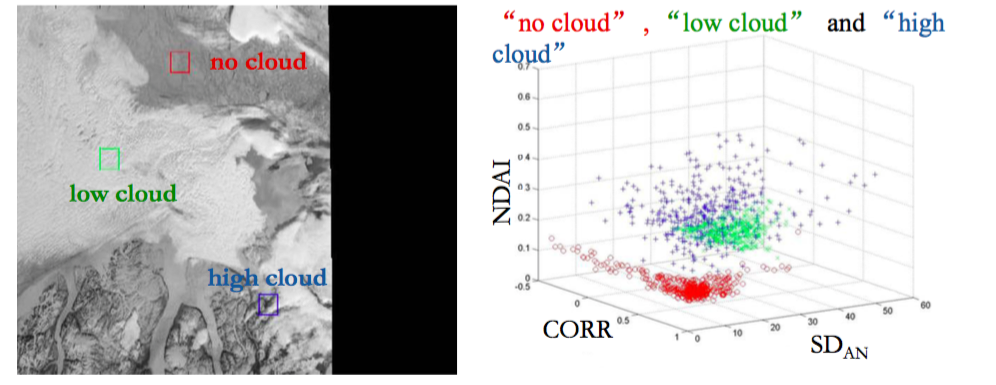
\includegraphics[scale=0.4]{ELCMC.png}
\end{center}
\caption{The ELCMC algorithm}
\label{fig:elcmc}
\end{figure}

